\documentclass{article}
\usepackage{amsmath} % equation, align, matrix, *, &, \\, \left, \right
\usepackage{graphicx} % figure
\usepackage{subcaption} % subfigure
\usepackage{comment} % To comment
\usepackage{hyperref} % To hyperlink and ref
\usepackage{enumitem} % To list
%\usepackage[ngerman]{babel}
\usepackage[utf8]{inputenc}
\usepackage{wrapfig}
\usepackage{ulem}
\usepackage[backend=bibtex,style=numeric]{biblatex}
\usepackage{subfiles} %multifile latex projects
\usepackage{multirow}
\usepackage{booktabs}
\usepackage{csquotes}
\usepackage[section]{placeins}
\usepackage{color,soul}

%\usepackage{fontspec}
\graphicspath{{images/}{../images/}}

\bibliography{lib} 

\title{IoT Project: \\Height / capacity monitor}
\author{Grupo K: \\ Tim Reiprich \\ Tegshigzugder Otgonbayar \\ Luca Maltagliati}

\begin{document}

\pagestyle{plain}
\pagenumbering{gobble} %hide page numbers

\maketitle
%\section{}
%\subsection{}
%\subsubsection{}

%\paragraph{}
%\subparagraph{}

\newpage

\textcolor{red}{\textbf{\hl{This documentation will be updated until the final delivery.}}}

\pagenumbering{arabic} %show page numbers in arabic
\tableofcontents % from the section headings
\newpage

%\listoffigures
%\listoftables
%\newpage

%\paragraph*{Lectura 1.- Capítulo 1 de Michael Miller (2015), "The Internet of Things: How Smart TVs, Smart Cars, Smart Homes, and Smart Cities Are Changing the World" , Que}\mbox{}\\

%\paragraph*{Project: Height / capacity monitor}\mbox{}\\

\section{Introduction}

In the project of the course Internet of Things we are to implement a device, that could be somewhat used in an environment. For this project we chose from the possible project ideas the Height / capacity monitor. We picked this idea, because it was interesting to see how it could be implemented and used in the field. Especially as we could think of certain sceneries, where it can be used efficiently such as, in household, for example where there are children to have such a sensor and turn the water off or even send a notification. In industrial area probably for indicators of highly valuable liquid. --- must be reformulated (maybe more industrial than household with children)

Our task was to create this device and also make it possible to connect with other 
For an inexpensive implementation we worked with the ESP8266. During the development we used the Arduino IDE and to easily create an user interface Node-Red was used.
\textcolor{red}{\textbf{\hl{Context and general summary of the operation of the system}}}

\section{Context and general description of the device}

Our project focuses on the measurement of containers holding some kind of liquid. Based on the volume of these containers alarms can be sent to the users to notify them about the amount. To accomplish this, a sensor will be used, that can determine the height of the liquid in the container. Furthermore an upper and a lower threshold can be set by the user. If one of these is exceeded, an alarm in form of a LED at the sensor and a virtual LED in Node-Red goes off.\par

\subsection{Hardware scheme}

\begin{figure}[h]
\hspace{-1cm}
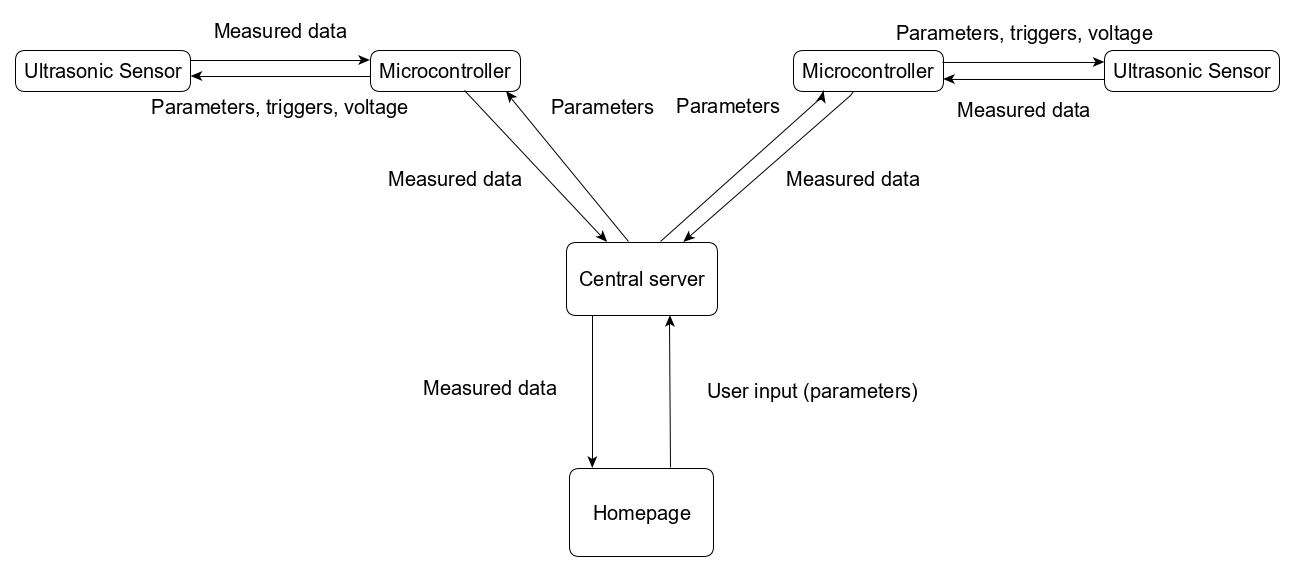
\includegraphics[scale=0.325]{images/circuit3.png}
\caption{Hardware scheme}
\label{scheme}
\end{figure}

The basic scheme of system hardware is described as follows: the main components
are a computer as central server, the sensors and a web-page. The
sensors must be able to connect to the server via a WiFi-connection and for this
we assume that the connection is robust and will be available in the given
environment. The homepage is hosted on the central server and functions as the main way to interact with the system for the enduser. In theory it wouldn't be difficult to expand the system to function with multiple height sensors as seen in figure \ref{scheme}. But due to restrictions in available components we implemented only one sensor communicating with the central server in the final project.\par

\subsection{Sensor}
We used an ultrasonic sensor to measure the level of the liquid. The one we used, is called Ultrasonic Sensor Module HC-SR-04 by Robokart. 
We want to choose this approach because it is one of the best ways to sense proximity and detect levels with high reliability. The sensor is connected to a microcontroller 
that collects the data and sends them to the central server via WiFi.  

Every container will have a microcontroller that is connected to at least one sensor (see figure \ref{sensorWithArduino}).
Certain specified heights of minimal and maximal volumes can be set dynamically, depending on various factors, like the position of the container, the probability of it being used, the liquid type and as such.

\begin{figure}[h]
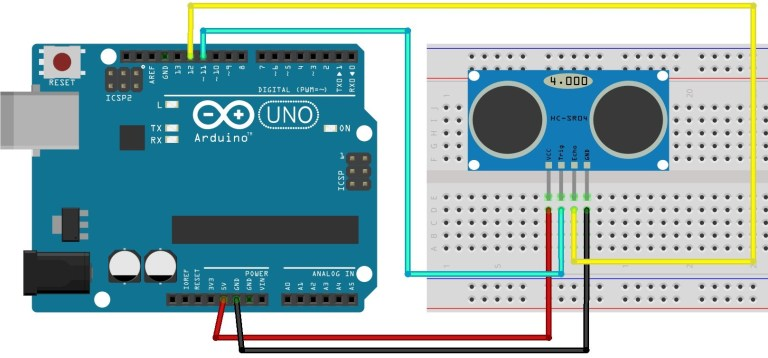
\includegraphics[scale=0.5]{sensorAndArduino.jpg}
\caption{Example of a sensor connected to a microcontroller}
\label{sensorWithArduino}
\end{figure}

\subsection{Central server}

We assume a LAN or WLAN network to which the controllers and central
server are connected. Through this the microcontrollers will be able to communicate with the central server by sending the measurements of the liquid heights continuously. 
The central server will perform checks on the thresholds curerntly set by the user and, if needed, will show an alarm on the homepage and send the alarm signal to the microcontroller connected to the sensor, so the alarm in form of the connected connected LEDs will be shown as well. This procedure and the corresponding homepage was configured using Node-Red.

\section{Steps of the project}

The first steps of the project consisted of research about similar projects and
identifying platforms, programming languages and frameworks, choosing
the most suitable ones for our case. Furthermore, the connection between devices plays a crucial role, so we needed to know what kind of protocols are needed.
During the next phase we planned the structure of the system and began to get familiar with the tools we wanted to use. After the planning was done we implemented the system and tested it afterwards to remove possibly found errors.\par 

\textcolor{red}{\textbf{\hl{Complete list of components that will be used, with a short description and why}}}

List of ordered components
\begin{itemize}
\item NodeMCU DevKit v1.0 development board (ESP8266) - we will use the microcontroller connected to sensor. It collects and sends data to broker and receives parameters to light up the warning LEDs correctly.
\item Ultrasonic proximity sensor (digital / analog output module) - the main sensor to measure the distance between liquid and sensor
\item power source for the microcontroller and sensor (batteries, solar panel or a similar source)
\item Small materials: 
	\begin{itemize}
		\item cables - to connect sensor, microcontroller and LEDs
		\item breadboard - to connect sensor, microcontroller and LEDs
		\item LEDs - to signal that level of liquid has exceeded height thresholds set by the user
		%push button - a button is always useful
	\end{itemize}
\end{itemize}

\begin{figure}[]
	\centering
	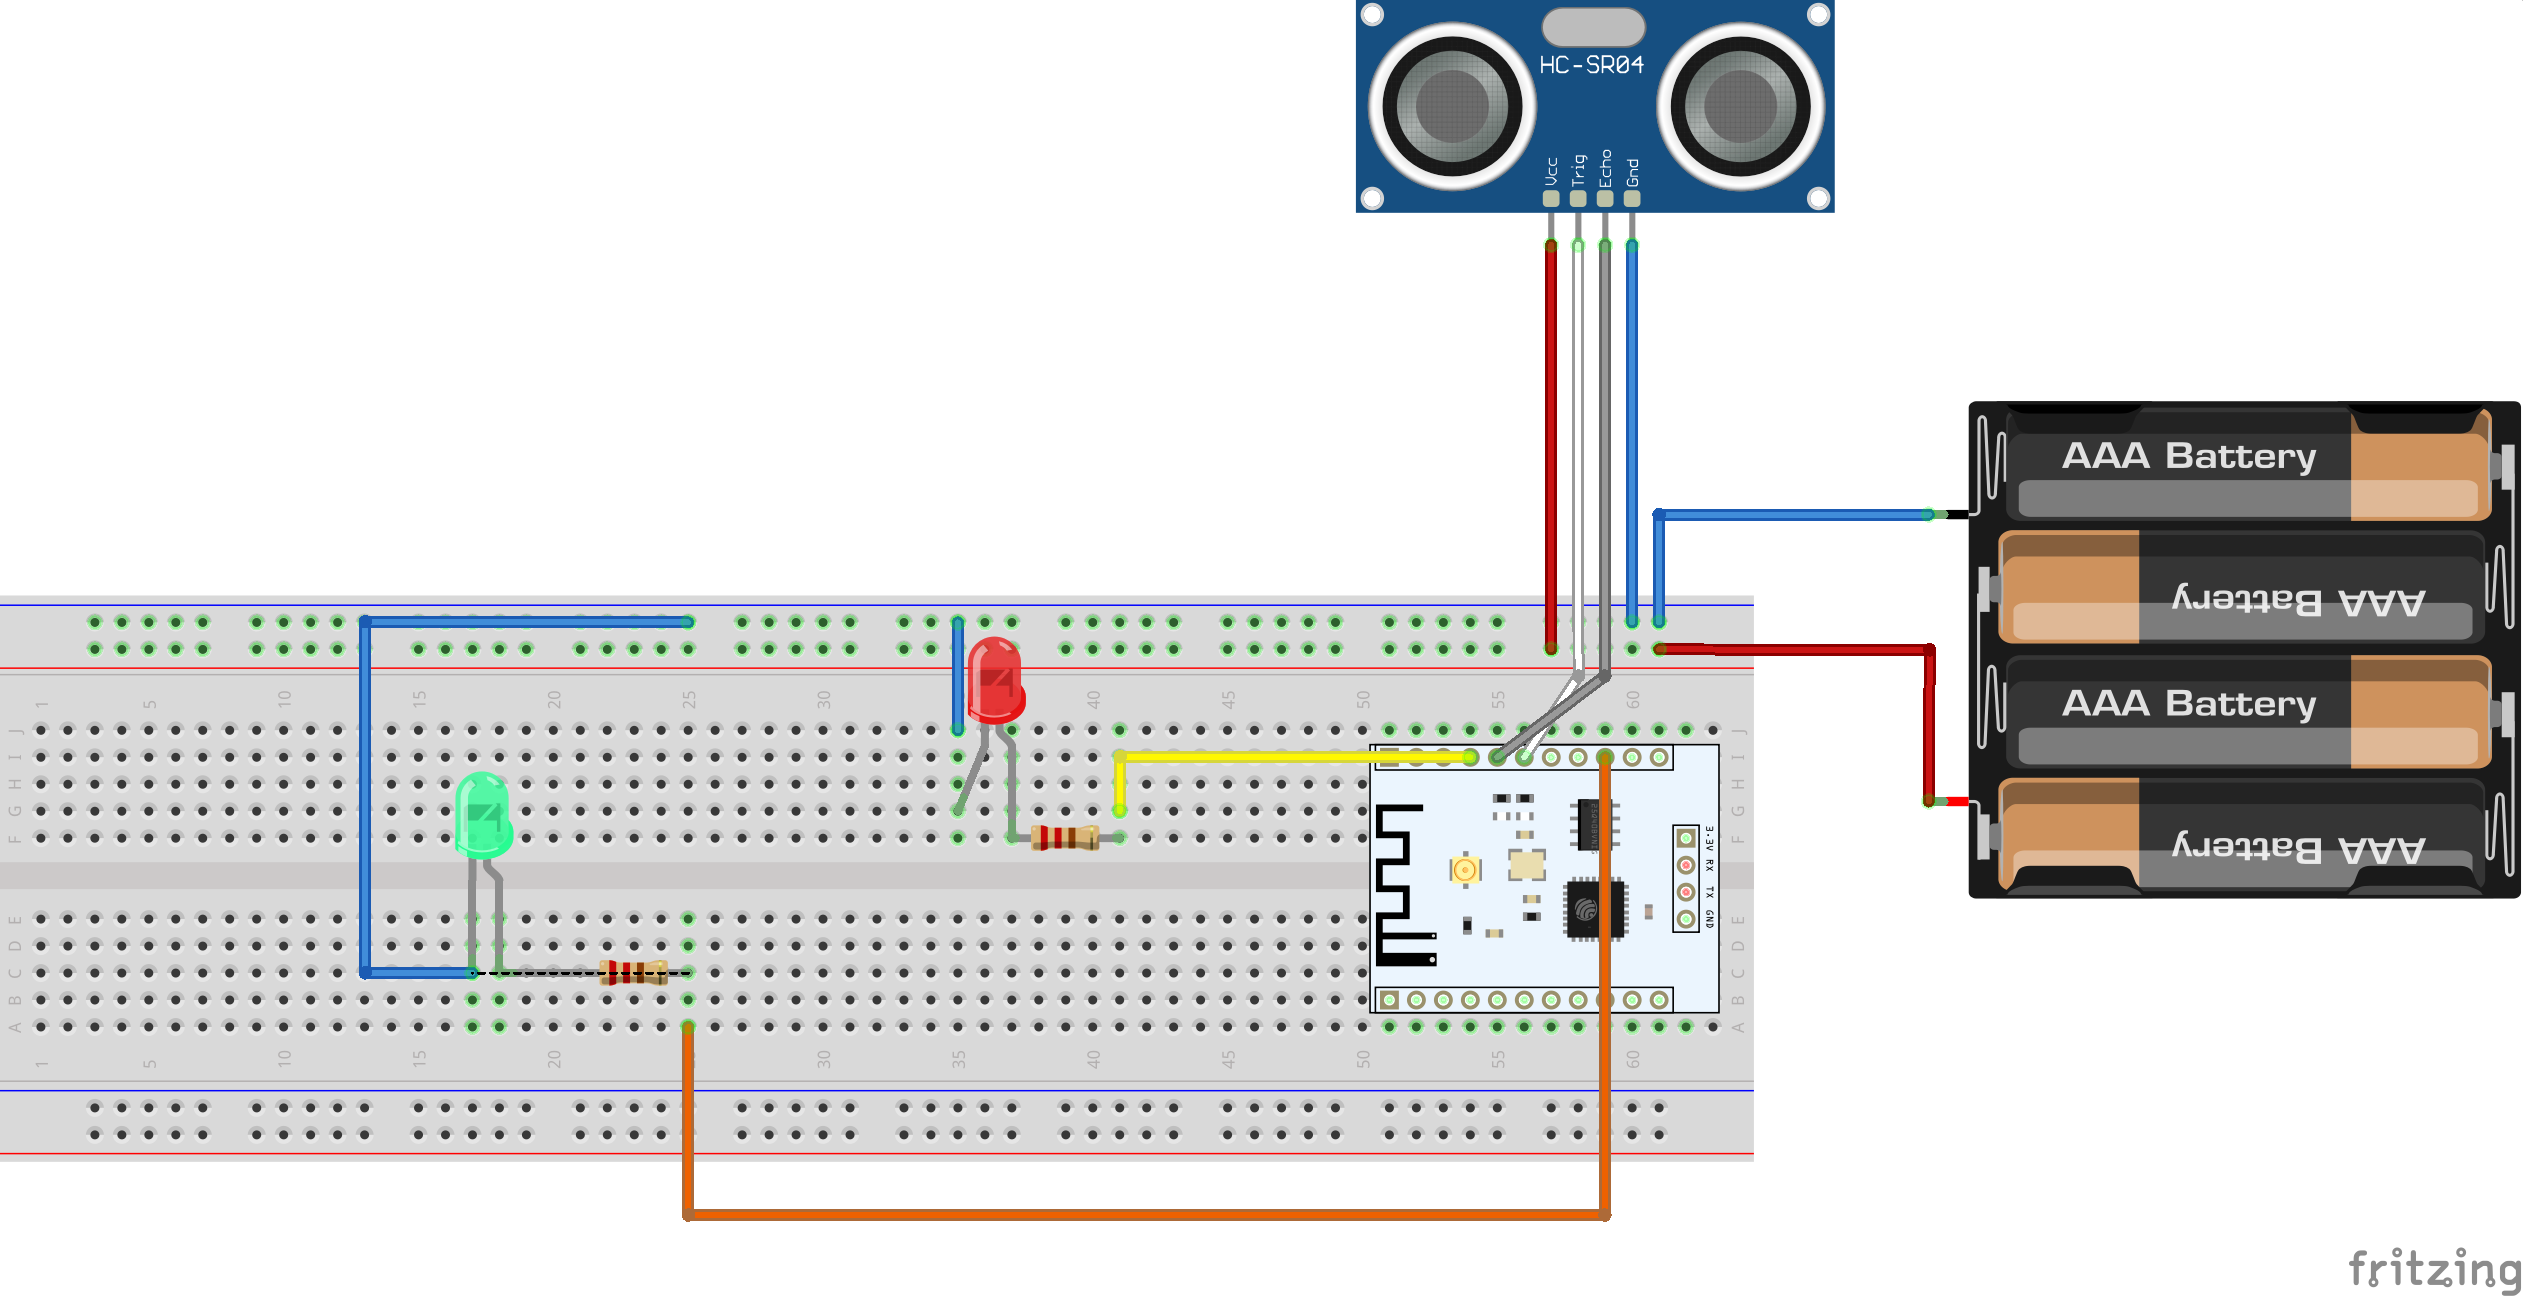
\includegraphics[scale=0.4]{images/schema_bb.png}
	\caption{Hardware scheme}	
	\label{schema_bb}
\end{figure}

\textcolor{red}{\textbf{\hl{Complete wiring scheme }}} - will be documented during the implementation 
\begin{itemize}
	 \item Flowchart of operation  
	\begin{figure}[h]
		\center
		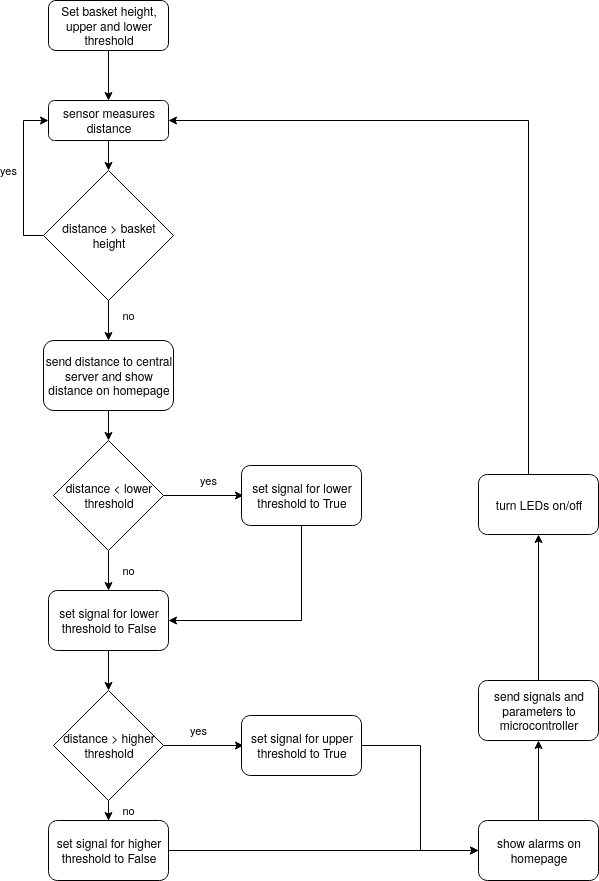
\includegraphics[scale=0.6]{flowChart.png}
		\caption{flow chart of the system}
		\label{sensorWithArduino}
	\end{figure}
	\item Another entry in the list
	
\end{itemize}

\textcolor{red}{\textbf{\hl{User manual:}}}
\begin{itemize}
	\item System installation, specifications and calibration
	\item System use and maintenance manual
	\item Detection and solution of possible errors
\end{itemize}

\subsection{Node-Red}
This section covers the parts of the project running on the central server which mainly includes the homepage created with Node-Red. The flow we created for this project can be seen in figure \ref{flowScheme} and the simple user interface in figure \ref{inteface_offline}. The flow consists of 4 input elements located on the left. Located in the middle of the flow there are nodes transforming the input data and on the right all the output nodes are located.\par 
\subsubsection{Input nodes}
3 out of the 4 input nodes are simple text nodes through which the user can set the basket height, lower and higher threshold. All 3 can be changed at any point even if the system is running. This may be needed in cases like the liquid in the basket changed and due to a higher density the basket can hold less than before, the sensor is used in a new basket or similar use cases. The basket height has to be set because the used ultrasonic sensor sometimes measures faulty values. So the basket height is used to filter them and prevent the microcontroller from sending them to the MQTT broker.\par
The other input node receives MQTT messages from the MQTT broker. It is subscribed to the topic \enquote{distance} to which the microcontroller publishes the measured distance.
\subsubsection{Transforming and output nodes}
The function node called \enquote{Thresholds} checks if the user given thresholds are valid. This means it checks if the lower threshold is lower or equal to the higher trehshold and the other way around. If this is the case the new values for lower and higher threshold are stored in\verb|conext.low| and \verb|context.high|. Furthermore the node returns \verb|{payload: {upper: context.high, lower: context.low}}| which is used by the two connected text nodes on the right side to show the user the currently set thresholds on the homepage.\par 
The function node \enquote{Threshold Check} does the same checks as the previously discussed node and also stores the current threshold values in a similar manner.  Additionally it also stores the last measured distance and uses it to check if one of the two thresholds is surpassed. In the end the object \verb|{payload: {highLed: <boolean>, lowLed: <boolean>,|\\
 \verb| basketHeight: context.basket}}| is returned where the property highLed or respectively lowLed is set to \enquote{true} if the corresponding threshold is surpassed. The last property always contains the currently set basket height. Afterwards this object is published to the topic \enquote{threshold} as a JSON using MQTT. The microcontroller is subscribed to this topic and uses the received values to turn its connected LEDs on or off and to filter abnormal measured distances.\par 
Besides that the returned object of the node \enquote{Threshold Check} is also used as input for the function node called \enquote{filterLow}. It simplifies the input and returns the object \texttt{\{payload: "high"|"low"|"between"\}} where the value is chosen depending on the object given as input. We used this so we can simply check for received string in the LED nodes afterwards in the flow to determine if the LEDs have be turned off or on.\par 
And finally the two ouput nodes on the top are used to show the measured distances. The text node just shows the last measured distance in centimeters. The node called \enquote{Distance} is a graph of the measured distances which enables the user to see the tendencies in the liquid level and mybe act before the critical thresholds are exceeded.
\subsubsection{User interface}
The user interface (figure \ref{inteface_offline}) is structured in 3 parts. On the left the current status of the system is shown meaning the current parameters of basketheight, lower and higher treshold. Also it contains the 3 status LEDs signalizing if one of the thresholds is surpassed or if the system is in a non-problematic state (shown by the green LED names \enquote{normal} being turned on).\par 
In the middle the measurements are shown. This part consists of the last mesured distance and a graph showing the changes during the last measurements. These values can only be seen if a microcontroller with an ultrasonic sensor is publishing its data. Otherwise the graph is blank and the message \verb|desconnectado| is shown instead of the last measurement.\par 
The right-most part contains all nodes that allow user input. Through these the user can set the basket height, lower and higher threshold. This can happen dynamically at any time. The changes will be published to the MQTT broker and therefore the microcontroller everytime one of the values is changed or after a new measurement arrives.
\begin{figure}
	\centering
	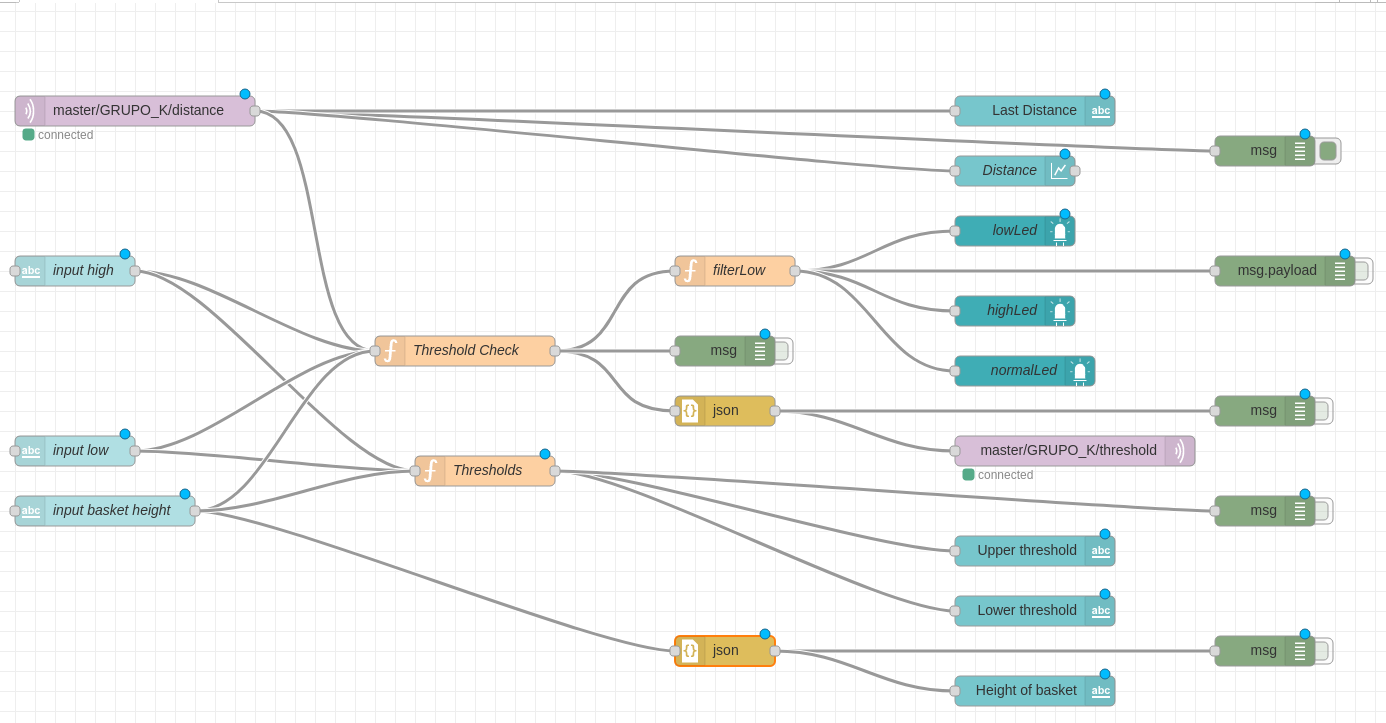
\includegraphics[scale=1.2]{images/flowScheme.png}
	\caption{Node-Red: Scheme of flow}	
	\label{flowScheme}
\end{figure}

\begin{figure}
	\centering
	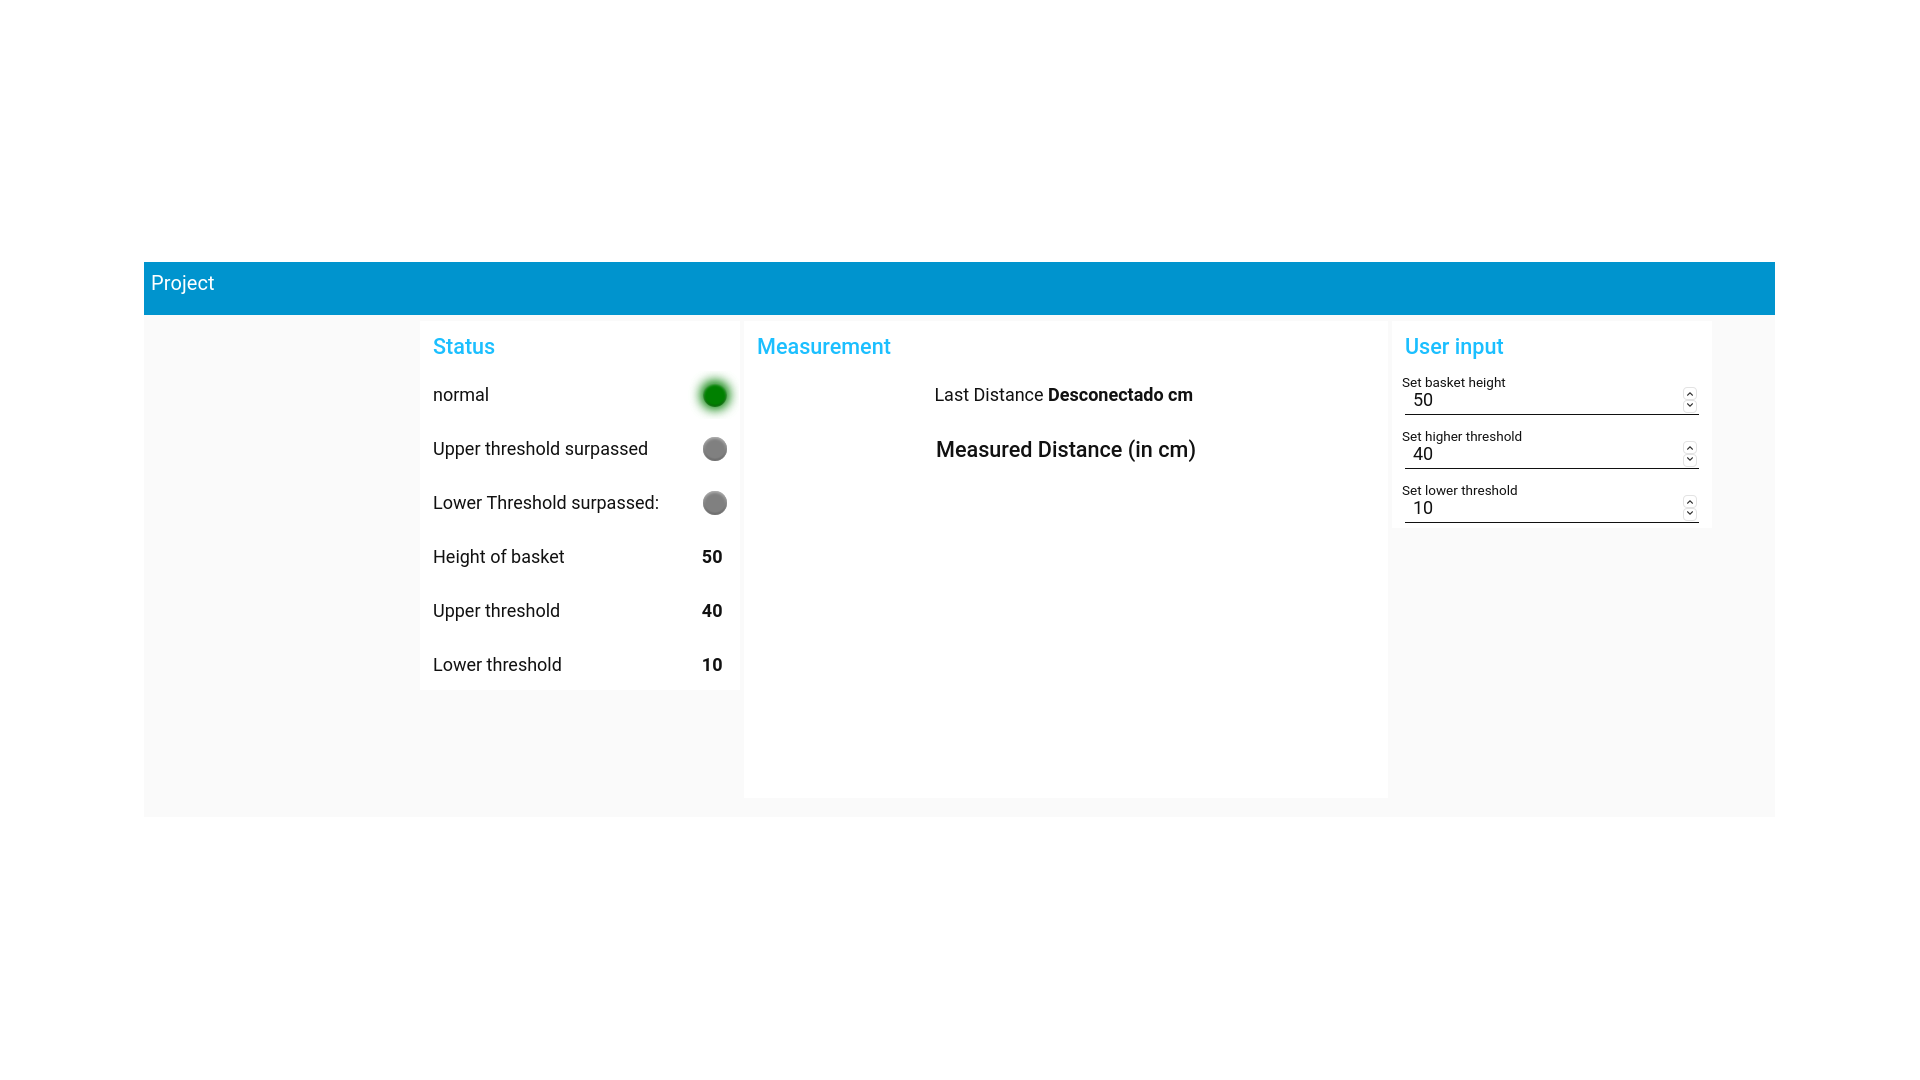
\includegraphics[scale=0.25]{images/interface_offline_2.png}
	\caption{Node-Red: Interface offline}	
	\label{inteface_offline}
\end{figure}
\subsection{Arduino IDE}
\begin{itemize}
\item List of functions used to communicate with the sensors, including input / output parameters and operation.
	\item List of functions that will be used to communicate with the base station, including input / output parameters and operation. 
	\item Other functions necessary for device operation
	\item Other technical considerations of the devices not described above. 
\end{itemize}

\section{Power Consumption}
During the last class we measured the power consumption of the system. The measurement happenend over a duration of $8.3$ seconds and the results can be seen in figure \ref{chart_power}.\par 
As seen in the graph the startup probably lasted around 3 seconds. In the beginning of it there are several spikes in power consumption. They could be the result of initial processes but we can't know for sure what is going on inside the ESP module. During $2.5$ and $3$ seconds there is a generally higher power consumption without big spikes. We think this is the period of time during which the ESP tries to establish a Wifi connection. Due to constant package traffic during this time a higher consumption could result.\par 
Afterwards there are a lot of spikes in power consumption which probably happened because the microcontroller periodically sends and receives data from the sensor which is sent together with other packages via Wifi. Another reason could also be if the connected LEDs are turned on or off but this is hard to tell given only this sample.\par 
If one wants to minimize the power consumption of the system, one could lower the frequency of mesurements performed by the sensor and therefore also the frequency of data exchange between the MQTT broker and the microcontroller. Also if the LEDs connected to the microcontroller aren't needed (because they are not visible or not important at the basket) they should be removed, so that the system becomes more efficient.

\begin{figure}[]
	\centering
	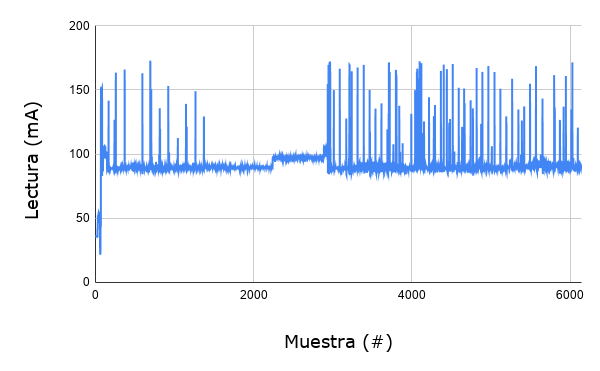
\includegraphics[scale=0.5]{images/chart.png}
	\caption{Hardware scheme}	
	\label{chart_power}
\end{figure}

\newpage

\section{Summary}
Through this project we were able to learn certain difficulties and also advantages of the ... 
There was new insight in how JSON BLA BLA 
In the future it would be interesting to study the capability of interconnecting with other devices and creating a more broad network of devices. Obviously it makes sense to work with: ...

\begin{comment}
Project : Height / capacity monitor
Using an ultrasonic sensor or similar, monitor the height of a water tank, paper stack, garbage container, or similar. Think of multiple sensors to map the height in different positions of the container or different containers. To properly manage the filling / emptying of the container, monitoring the tank capacity, etc. Local warning by LEDs, minimum / maximum level alarms, etc.

How is the document going to be valued?

Well written and clear
	Good: The document has no misspellings, and a simple language is used that is perfectly understood. The document is careful: it looks nice, the sheets, drawings, etc., are numbered, the different sections are clearly marked. It shows that they have taken it seriously.
	Enough: The document is understood quite well, although there is some part that can be improved. I found some error, probably attributable to a mistake. With a little more effort, it could have been better.
	Insufficient: I have found several spelling mistakes, and I have not understood many of the things that are said in the document. The document is quite neglected. It shows that they have not tried very hard.


Adequate content
	Good: The document includes complete information on all the points that were requested. They also explain and briefly justify the decisions made.
	Enough: The document includes all the points, but the information is not complete in no more than three of them, or some point is missing. I see some dark aspects in the description of some point. Some key decisions are not justified
	Insufficient: More than one point is missing or the description is quite incomplete 


Good and effective approach
	Good: The approach is good. I can't think of many improvements. The scheme and operation is clear and reasonable. The functions that will be used are well described, with a clear comment on what they do. With this information I think that I would have no difficulty in making the design myself.
	Enough: I think the proposal is good although it admits some improvements. I understand well what they want to do, but if I had to implement it, I would have to ask for some additional clarification.
	Insufficient: The approach is not good. I do not understand the purpose or need of some of the elements of the structures, or of some of the procedures and functions. If I had to implement the application, with this information I would not know where to start.

\end{comment}

\begin{comment}
\maketitle
\newpage

\pagenumbering{arabic} %show page numbers in arabic
\tableofcontents % from the section headings
\newpage

\listoffigures
 
\listoftables

%\listoftables
\newpage

\subfile{einleitung/einleitung}
\newpage

\subfile{grundlagen/grundlagen}
\newpage

\subfile{analyse/analyse}
\newpage

\printbibliography

\subfile{entwicklung/entwicklung}
\newpage

\subfile{evaluation/evaluation}
\newpage

\subfile{zusammenfassungundausblick/zusammenfassungundausblick}
\newpage

\end{comment}

\end{document}